\section{Proposed architecture}
Our mushroom classification model utilizes the EfficientNetB0 architecture, renowned for its efficiency and performance in image classification tasks. Fine-tuning the pre-trained EfficientNetB0 model on our dataset allows it to adapt its parameters to the specific task of mushroom classification while leveraging knowledge learned from large-scale image datasets.
EfficientNetB0 is a unique convolutional neural network architecture because it prioritizes computational efficiency above performance to get cutting-edge results. To achieve that state of the art result, it proposes a few new ideas:
\begin{figure}[!ht]
    \centering
    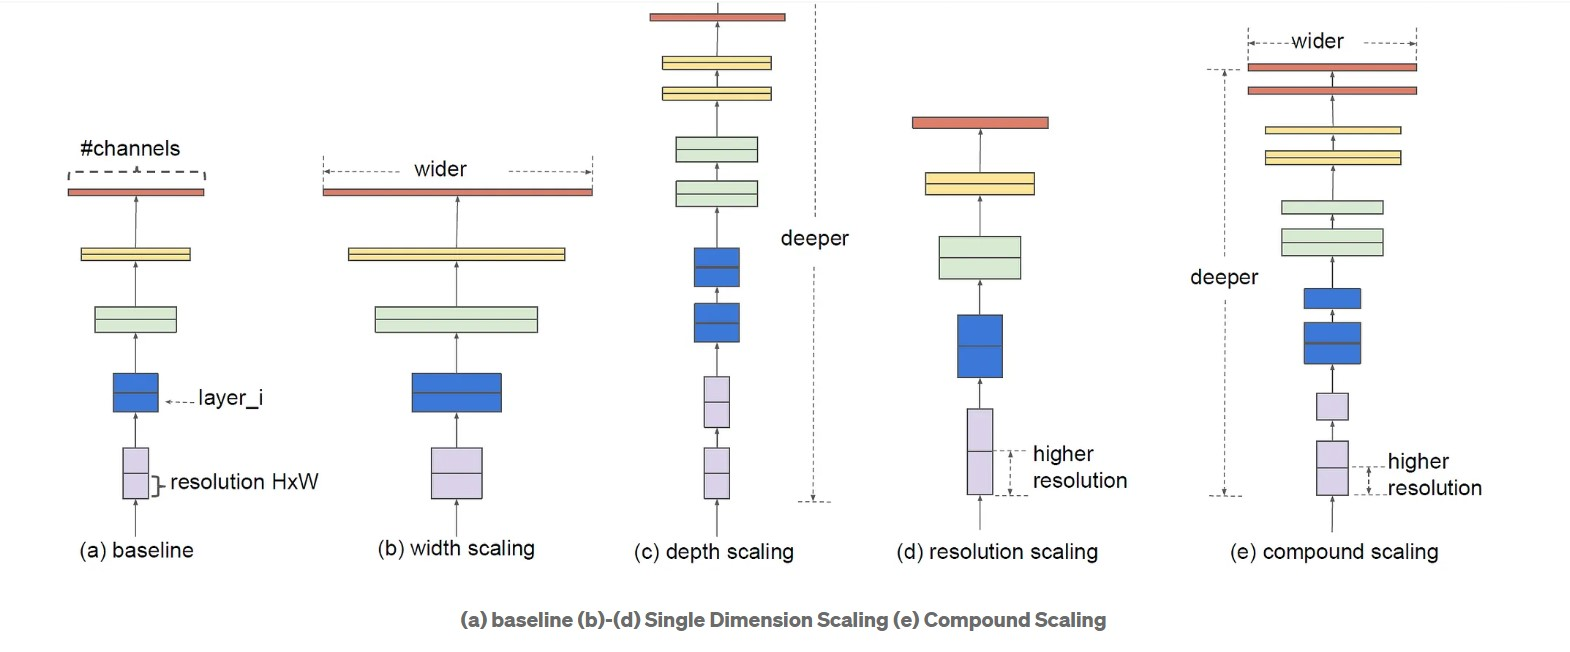
\includegraphics[height=6cm, width=9cm]{images/effwork.jpg}
    \caption{Figure 3 from Tan and Le (2020) illustrates the working of EfficientNetBO}
\end{figure}
\begin{enumerate}
  \item \textbf{Compound Scaling:} By uniformly scaling the model's width, depth, and resolution with a set ratio, this novel approach guarantees a balanced adjustment of these dimensions. With this approach, the model's performance is maximized without incurring exponentially higher computing costs\cite{tan2020efficientnet}.
  
  \item \textbf{Depthwise Separable Convolution:} EfficientNetB0 uses fewer computations and parameters than typical convolutional layers since it uses depthwise separable convolutional layers. This simplified architecture maintains representational capability while improving computing efficiency\cite{tan2020efficientnet}.
  
  \item \textbf{Inverted Residual Blocks:} EfficientNetB0 integrates inverted residual blocks with linear bottlenecks, drawing inspiration from MobileNetV2. These building components enable effective information transfer across the network, reducing computing burden and preserving high-quality feature representation\cite{tan2020efficientnet}.
  
  \item \textbf{Efficient Channel Attention (ECA):} By recalibrating channel-wise answers, ECA provides a lightweight technique for channel attention, improving feature representation. This addition increases the efficiency of the model by supporting its performance without dramatically increasing computational expenses\cite{tan2020efficientnet}.
  
  \item \textbf{Swish Activation Function:} Using this activation function, which has smoother behavior than more conventional activation functions like ReLU, allows EfficientNetB0 to operate more efficiently. This decision preserves computational economy while improving performance on a variety of jobs\cite{tan2020efficientnet}.
  
  \item \textbf{Model Scaling:} The compound coefficient ($\phi$) was introduced to allow for scalable model design. This means that practitioners can adjust the size of the model according to the computational resources that are available and the performance levels that they want\cite{tan2020efficientnet}.
\end{enumerate}


EfficientNet architecture consists of seven blocks which are shown in different colours. The basic building block of EfficientNet-B0 is a mobile inverted bottleneck convolution (MBConv), while each MBConv block is shown with the corresponding kernel filter size \cite{zhou2022multihead}. The figure below shows the different block:

\begin{figure}[!ht]
    \centering
    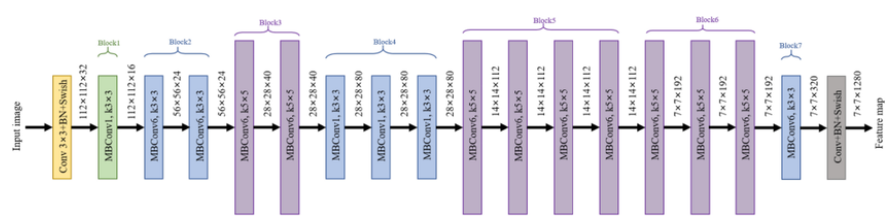
\includegraphics[height=6cm, width=9cm]{images/efflayer.PNG}
    \caption{Figure 3 from Zhou et al. (2022) illustrates the architecture of EfficientNetBO}
\end{figure}

The model comprises convolutional layers followed by depthwise separable convolutions. We modify this EfficientNetB0 by adding few layers and a classification layer. Global average pooling was used to reduce the parameter size. This layer not just reduce parameter also preserve the most important features by taking out the average. On top of that dense layer with ReLU activation was used further enhancing the model's ability to learn complex pattern in images, dropout regularization was used ensuring that the model could be generalized and does better on test set rather than just doing good only on training set. And a classification layer with sigmoid activation was used for binary classification. This architecture enables the development of a robust classification model capable of accurately distinguishing between edible and poisonous mushrooms.